%--------------------------HOLE-------------------------------
% Что это?
% Это файл с простым текстом( выводы, описание чего-либо), который редактируются вручную.
% Описание (для чего файл):введение
% Hole number:1

Цель работы: исследование скользящих режимов в системах с переменной структурой методом фазовой плоскости.
\subsection{Общие сведения}
\subsubsection{Система с переменной структурой}
Применение систем с переменной структурой позволяет получить высокое быстродействие,
 т. е. протекание процессов за минимальное время при
незначительных колебаниях, а в отдельных случаях и при отсутствии 
колебаний выходных координат в установившихся режимах. В работе рассматривается два варианта движений
в системе с переменной структурой,
которые в общем случае могут быть
представлены на рис.\ref{fig:example1}, где введены следующие
 обозначения: ОУ – объект управления; УП – устройство переключения; 
 $k_1$ и $k_2$ – коэффициенты регулятора.

\begin{figure}[!h]
\begin{subfigure}[b]{0.5\linewidth}
	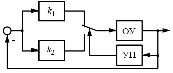
\includegraphics[width=\linewidth]{images/example1}
	\caption{ Система с переменной структурой.}\label{fig:example1}
\end{subfigure}
\begin{subfigure}[b]{0.4\linewidth}
	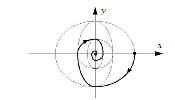
\includegraphics[width=\linewidth]{images/example2}
	\caption{ Фазовые траектории системы
		с переменной структурой.}\label{fig:example2}
\end{subfigure}
\caption{}\label{fig:example3}
\end{figure}
Пример движения
изображающей точки на фазовой плоскости  показан на рис.\ref{fig:example2}.
 Из приведенного рисунка следует, что система становится
асимптотически устойчивой, но устойчивого положения равновесия она достигает только при $t\rightarrow\infty$.

\begin{table}[!h] \centering
	\caption{ Таблица вариантов.} \label{tab:tab1}
	\begin{tabular}{|c|c|}
		\hline
		Вариант & 3\\ \hline
		k &  3.5 \\ \hline
	\end{tabular}
\end{table} 
	Допустим, объект управления – это система второго порядка, не обладающая при постоянной структуре собственной устойчивостью. Математическое описание системы \eqref{eq:eq1} .
	\begin{equation}\label{eq:eq1}
	\text{\"{x}}+k\,\text{x}=0
	\end{equation}
	Задание варианта указано в табл.\ref{tab:tab1} .





